
\section{Results}
\subsection{Experimentation}
\begin{frame}
  All experiments were evaluated in a Lanix Spine BW
  Processor Intel Xenon, CPU E5-2867W, 3.10 GHz.
  With operative system Ubuntu 14.04.3 LTS
  The models were solved with CPLEX 12.6.0.0,
  and they were coded in C++.
\end{frame}

\begin{frame}
  Different random instances were generated
  to validate the proposed formulations.
  For $n = 100$ we created 3 instances with $m = 20,30,40$,
  and different values of $p$, shown in the following table.
  \begin{table}
    \centerign
    \begin{tabular}{|c|c|c|}\hline
      n & m & p \\ \hline
      100 & 20 & 5-18 \\
      100 & 30 & 7-25 \\
      100 & 40 & 9,10 \\
      \hline
    \end{tabular}
  \end{table}
  
  The Model A was solved to optimality for all the values of $p$ when $m = 20$,
  for the rest of the values of $m$, none optimal solution was reported in less than one hour.

  The Model B was tested with each combination of $n,m,p$ and $\ell$ from $1,\ldots,p$.

\end{frame}

\begin{frame}
  Relation of $\frac{\ell}{p}$ versus the solution time.
  \begin{center}
    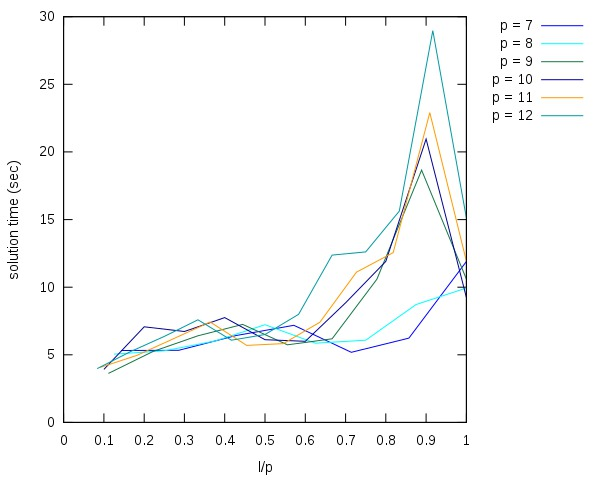
\includegraphics[scale=0.25]{grafica_01}
    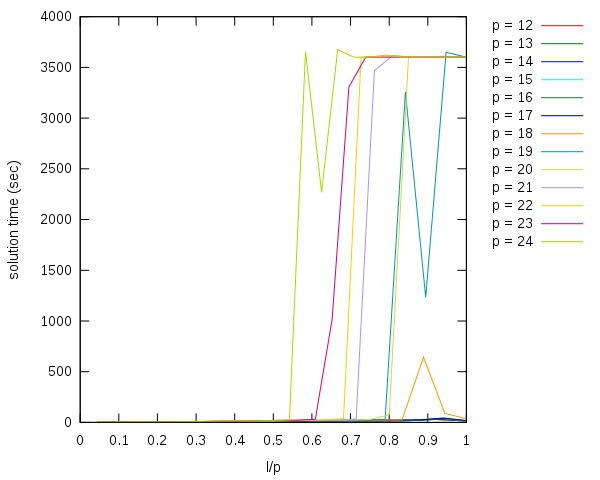
\includegraphics[scale=0.25]{grafica_02}
  \end{center}
\end{frame}

\begin{frame}

  The solution times increase drastically as $\ell$ approximates to $p$
  
  \begin{center}
    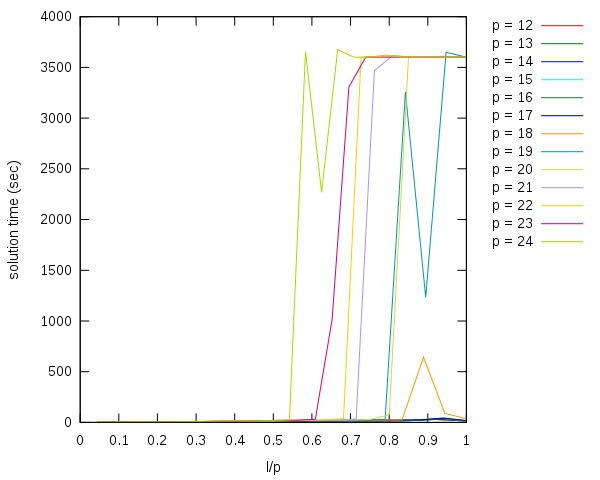
\includegraphics[scale=0.25]{grafica_02}
    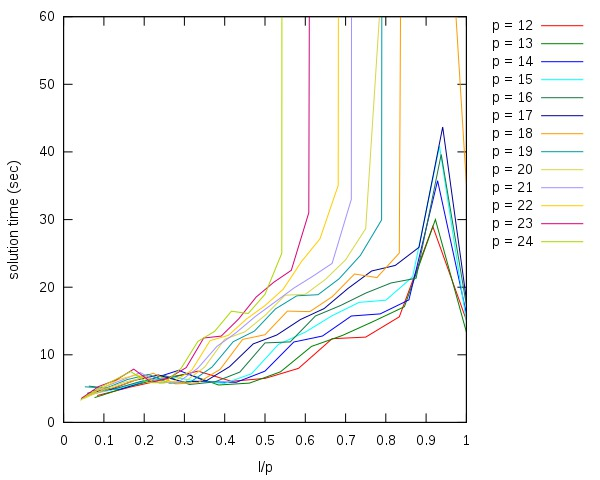
\includegraphics[scale=0.25]{grafica_03}
  \end{center}
  
\end{frame}

\begin{frame}

  For medium values of $p$, the value of the objective function does not change
  for medium/small to large values of $\ell$, were the optimal solution is obtained.

  \begin{center}
    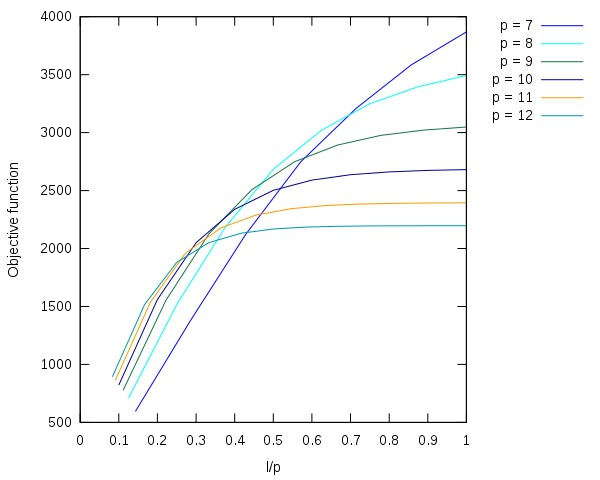
\includegraphics[scale=0.25]{grafica_04}
    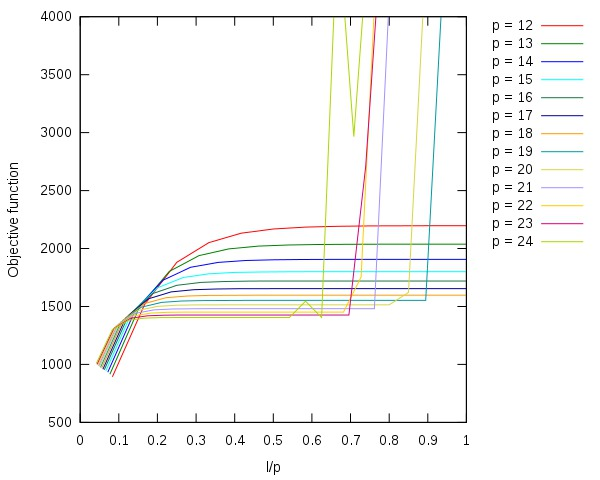
\includegraphics[scale=0.25]{grafica_05}
  \end{center}
  
\end{frame}

%% Caso 100 30 12
\frame{\begin{figure}[h!]\centering{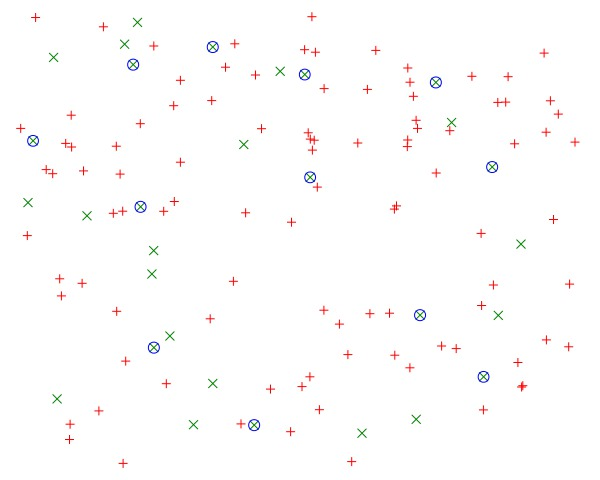
\includegraphics[scale=0.35]{Test_100_30_12_01}\caption{n = 100, m = 30, p = 12, l = 1}}\end{figure}}
\frame{\begin{figure}[h!]\centering{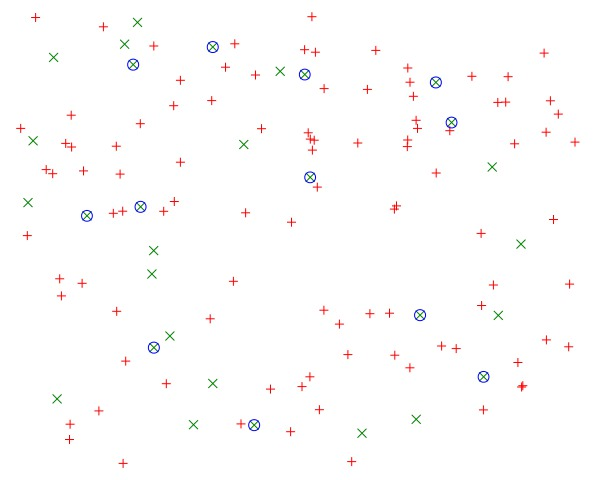
\includegraphics[scale=0.35]{Test_100_30_12_02}\caption{n = 100, m = 30, p = 12, l = 2}}\end{figure}}
\frame{\begin{figure}[h!]\centering{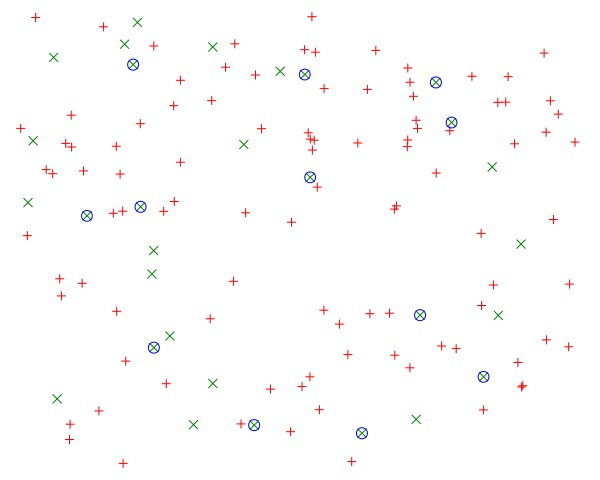
\includegraphics[scale=0.35]{Test_100_30_12_03}\caption{n = 100, m = 30, p = 12, l = 3}}\end{figure}}
\frame{\begin{figure}[h!]\centering{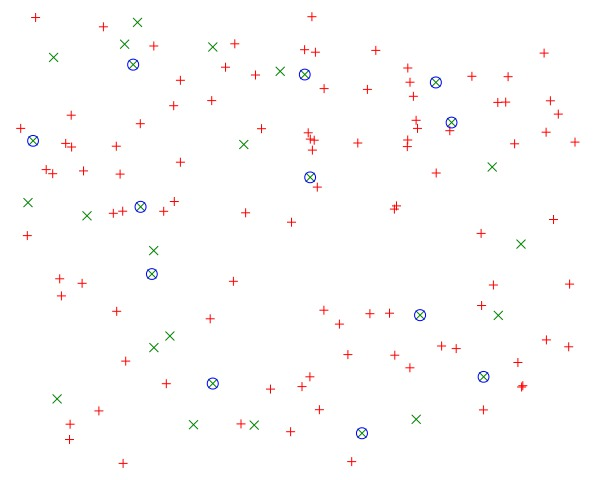
\includegraphics[scale=0.35]{Test_100_30_12_04}\caption{n = 100, m = 30, p = 12, l = 4}}\end{figure}}
\frame{\begin{figure}[h!]\centering{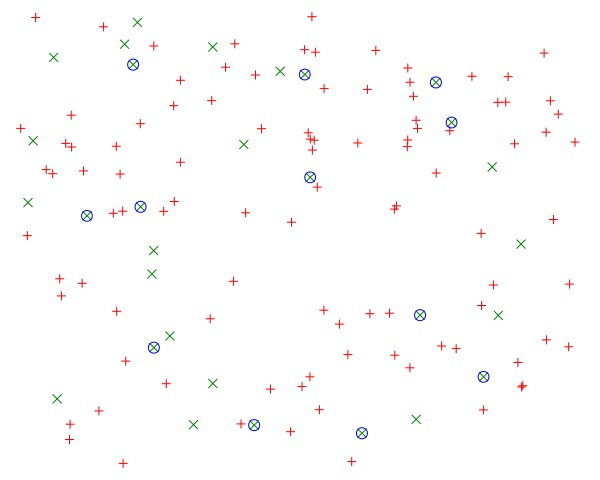
\includegraphics[scale=0.35]{Test_100_30_12_05}\caption{n = 100, m = 30, p = 12, l = 5}}\end{figure}}
\frame{\begin{figure}[h!]\centering{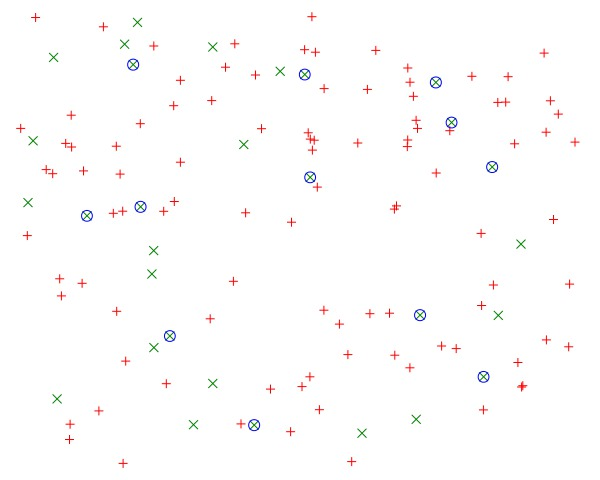
\includegraphics[scale=0.35]{Test_100_30_12_06}\caption{n = 100, m = 30, p = 12, l = 6}}\end{figure}}
\frame{\begin{figure}[h!]\centering{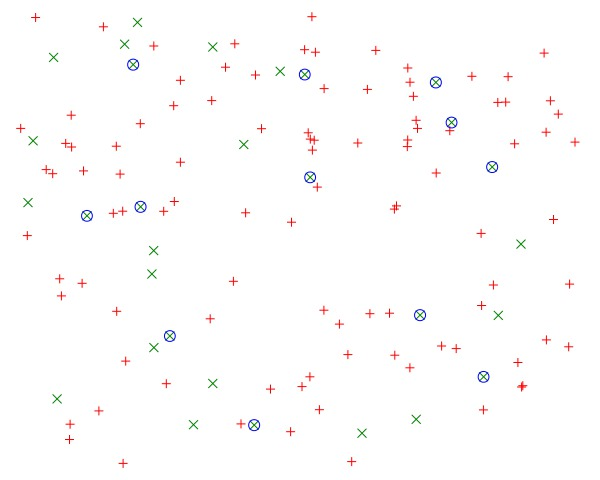
\includegraphics[scale=0.35]{Test_100_30_12_07}\caption{n = 100, m = 30, p = 12, l = 7}}\end{figure}}
\frame{\begin{figure}[h!]\centering{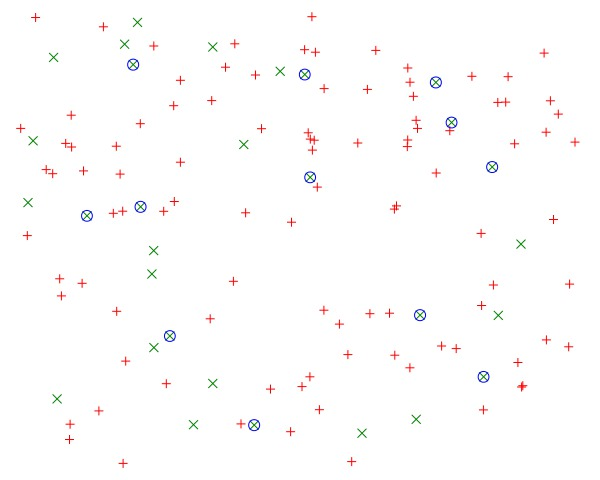
\includegraphics[scale=0.35]{Test_100_30_12_08}\caption{n = 100, m = 30, p = 12, l = 8}}\end{figure}}
\frame{\begin{figure}[h!]\centering{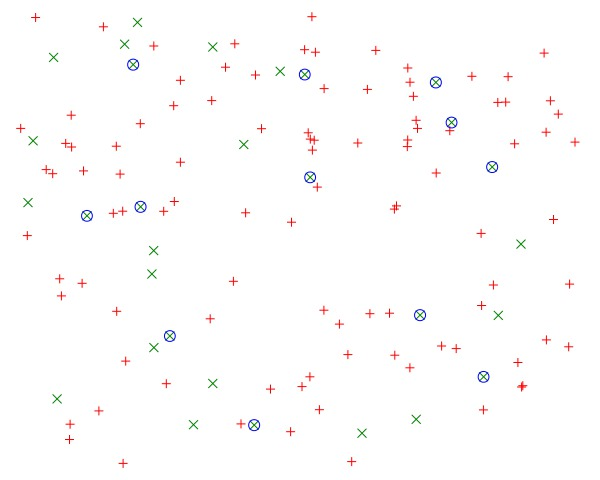
\includegraphics[scale=0.35]{Test_100_30_12_09}\caption{n = 100, m = 30, p = 12, l = 9}}\end{figure}}
\frame{\begin{figure}[h!]\centering{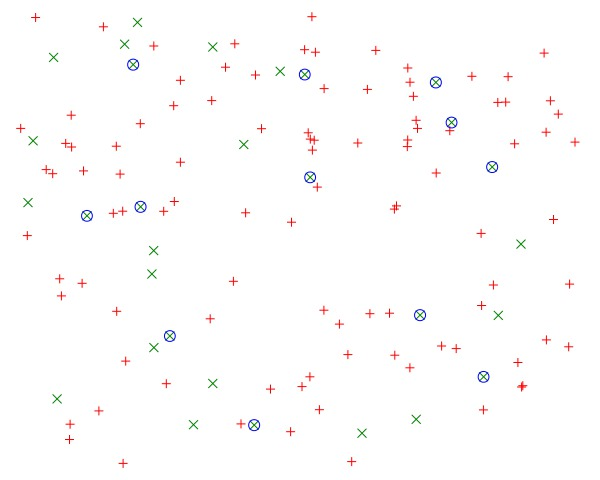
\includegraphics[scale=0.35]{Test_100_30_12_10}\caption{n = 100, m = 30, p = 12, l = 10}}\end{figure}}
\frame{\begin{figure}[h!]\centering{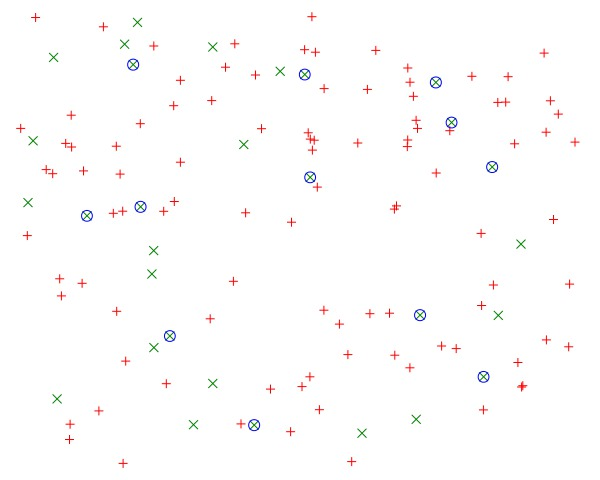
\includegraphics[scale=0.35]{Test_100_30_12_11}\caption{n = 100, m = 30, p = 12, l = 11}}\end{figure}}
\frame{\begin{figure}[h!]\centering{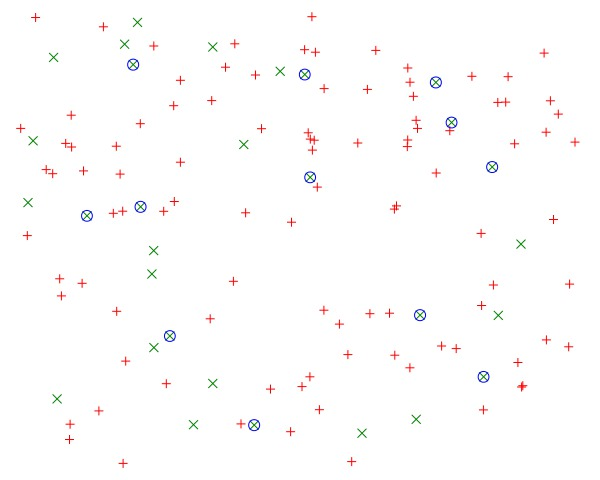
\includegraphics[scale=0.35]{Test_100_30_12_12}\caption{n = 100, m = 30, p = 12, l = 12}}\end{figure}}

\frame{\begin{figure}[h!]\centering{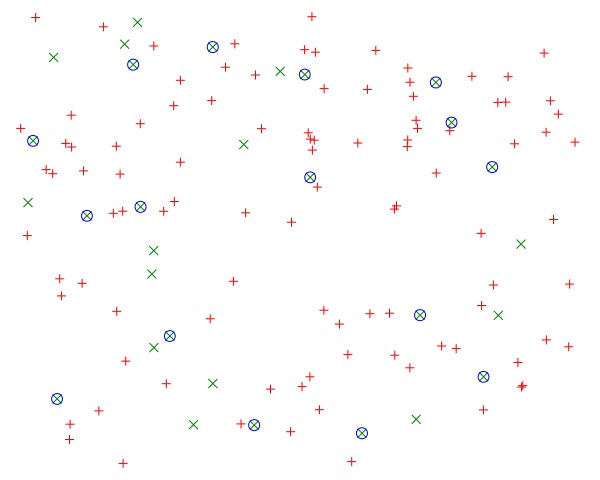
\includegraphics[scale=0.35]{Test_100_30_16_01}\caption{n = 100, m = 30, p = 16, l = 1}}\end{figure}}
\frame{\begin{figure}[h!]\centering{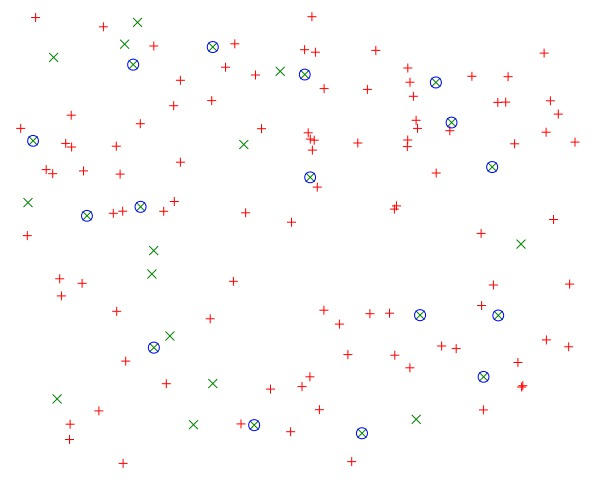
\includegraphics[scale=0.35]{Test_100_30_16_02}\caption{n = 100, m = 30, p = 16, l = 2}}\end{figure}}
\frame{\begin{figure}[h!]\centering{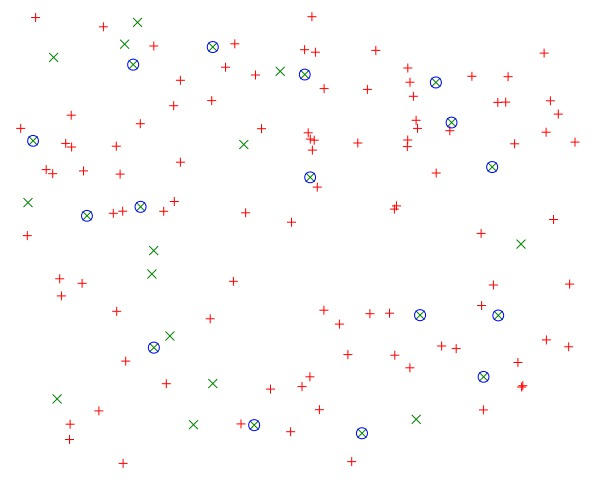
\includegraphics[scale=0.35]{Test_100_30_16_03}\caption{n = 100, m = 30, p = 16, l = 3}}\end{figure}}
\frame{\begin{figure}[h!]\centering{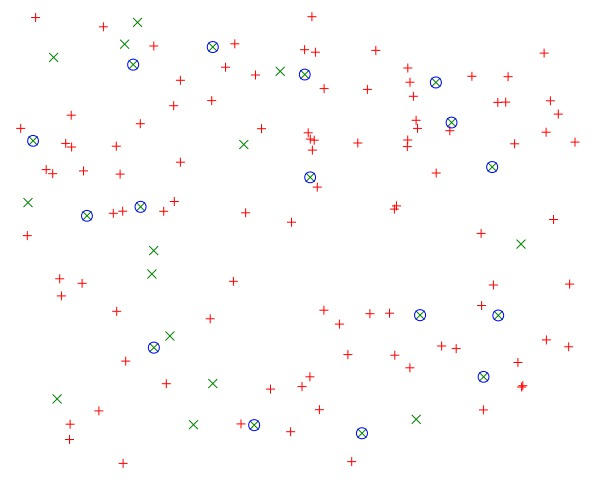
\includegraphics[scale=0.35]{Test_100_30_16_04}\caption{n = 100, m = 30, p = 16, l = 4}}\end{figure}}
\frame{\begin{figure}[h!]\centering{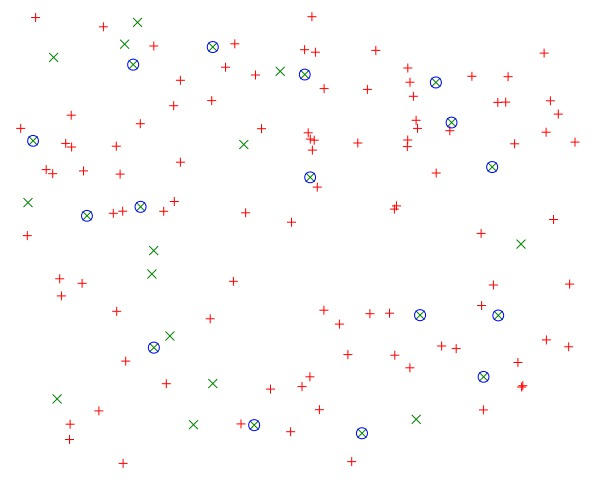
\includegraphics[scale=0.35]{Test_100_30_16_05}\caption{n = 100, m = 30, p = 16, l = 5}}\end{figure}}
\frame{\begin{figure}[h!]\centering{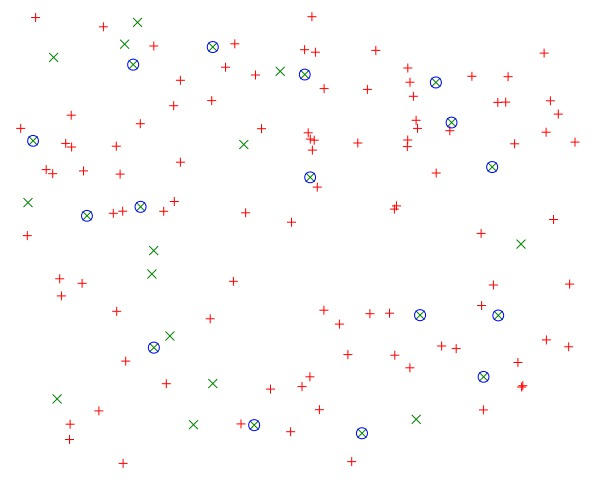
\includegraphics[scale=0.35]{Test_100_30_16_06}\caption{n = 100, m = 30, p = 16, l = 6}}\end{figure}}
\frame{\begin{figure}[h!]\centering{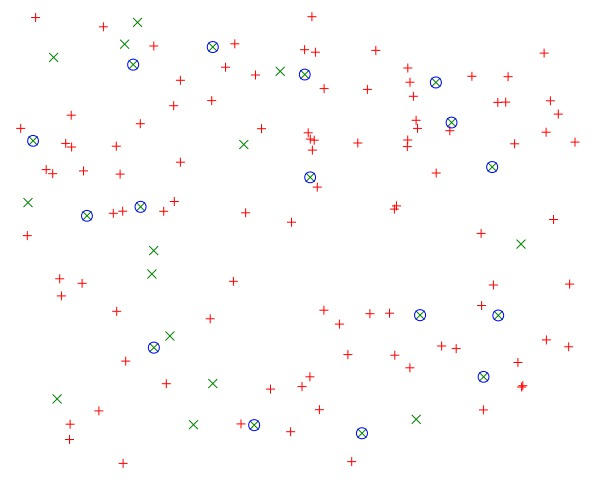
\includegraphics[scale=0.35]{Test_100_30_16_07}\caption{n = 100, m = 30, p = 16, l = 7}}\end{figure}}
\frame{\begin{figure}[h!]\centering{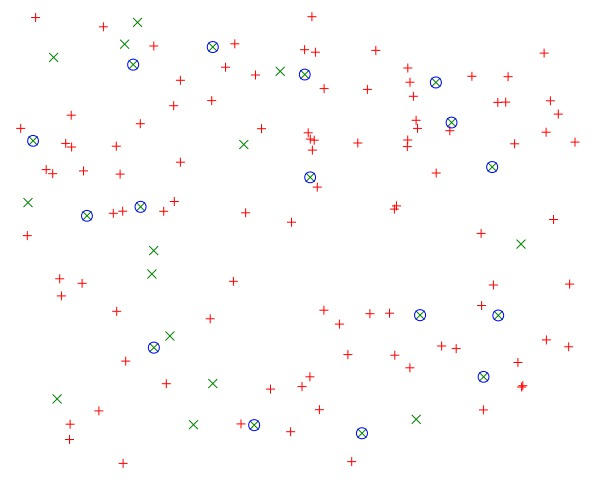
\includegraphics[scale=0.35]{Test_100_30_16_08}\caption{n = 100, m = 30, p = 16, l = 8}}\end{figure}}
\frame{\begin{figure}[h!]\centering{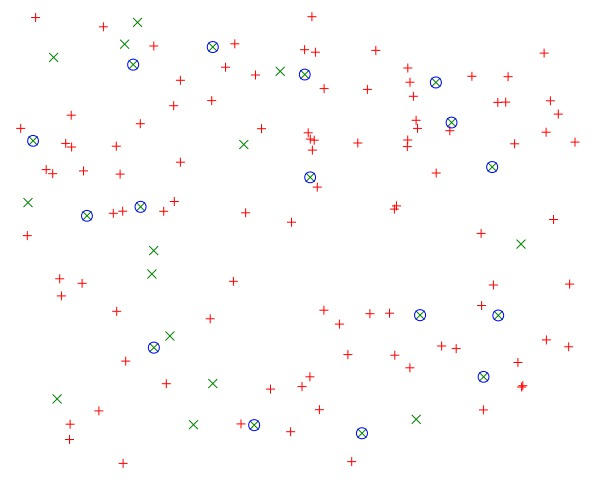
\includegraphics[scale=0.35]{Test_100_30_16_09}\caption{n = 100, m = 30, p = 16, l = 9}}\end{figure}}
\frame{\begin{figure}[h!]\centering{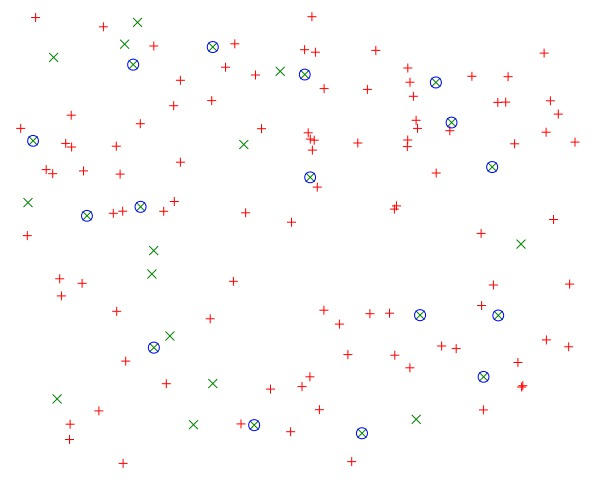
\includegraphics[scale=0.35]{Test_100_30_16_10}\caption{n = 100, m = 30, p = 16, l = 10}}\end{figure}}
\frame{\begin{figure}[h!]\centering{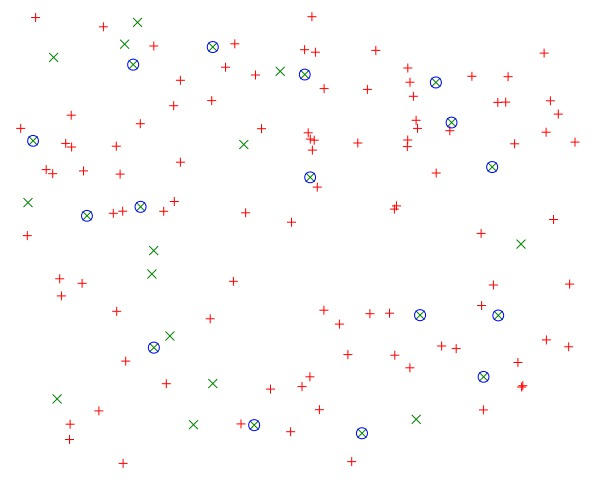
\includegraphics[scale=0.35]{Test_100_30_16_11}\caption{n = 100, m = 30, p = 16, l = 11}}\end{figure}}
\frame{\begin{figure}[h!]\centering{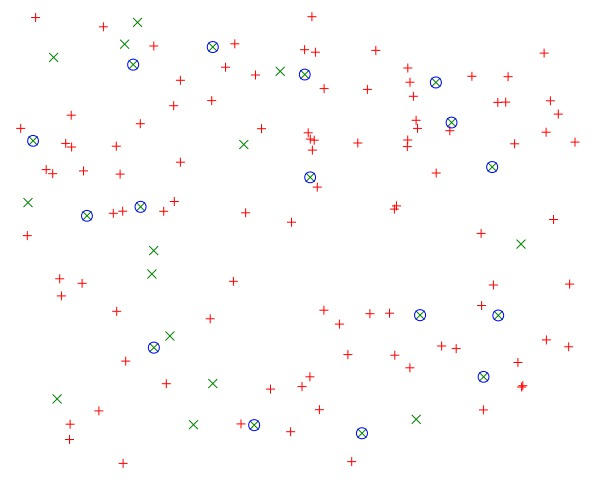
\includegraphics[scale=0.35]{Test_100_30_16_12}\caption{n = 100, m = 30, p = 16, l = 12}}\end{figure}}
\frame{\begin{figure}[h!]\centering{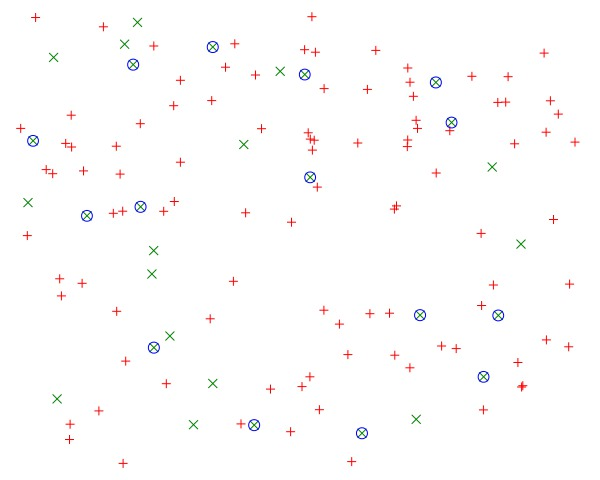
\includegraphics[scale=0.35]{Test_100_30_16_13}\caption{n = 100, m = 30, p = 16, l = 13}}\end{figure}}
\frame{\begin{figure}[h!]\centering{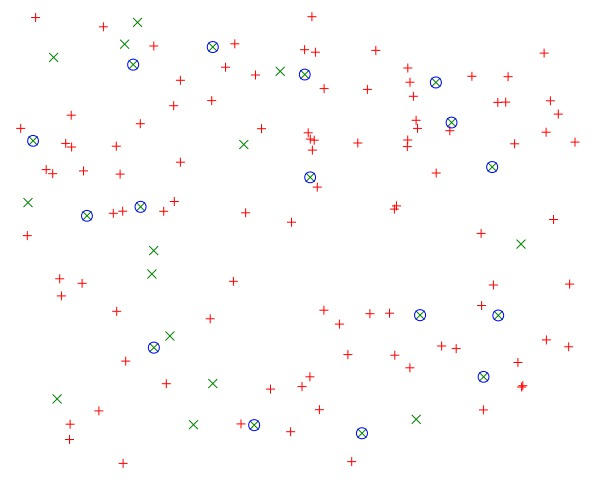
\includegraphics[scale=0.35]{Test_100_30_16_14}\caption{n = 100, m = 30, p = 16, l = 14}}\end{figure}}
\frame{\begin{figure}[h!]\centering{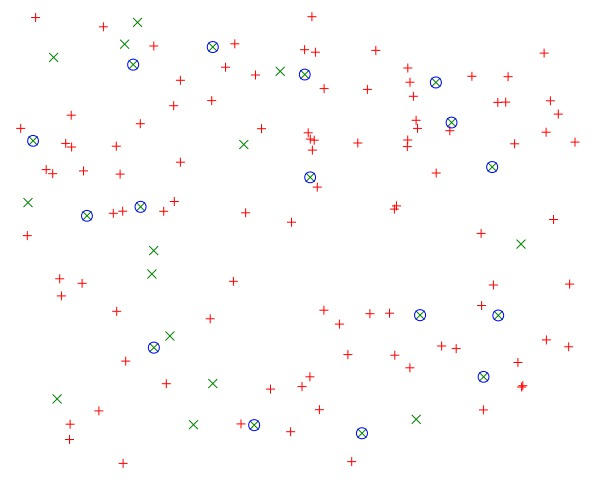
\includegraphics[scale=0.35]{Test_100_30_16_15}\caption{n = 100, m = 30, p = 16, l = 15}}\end{figure}}
\frame{\begin{figure}[h!]\centering{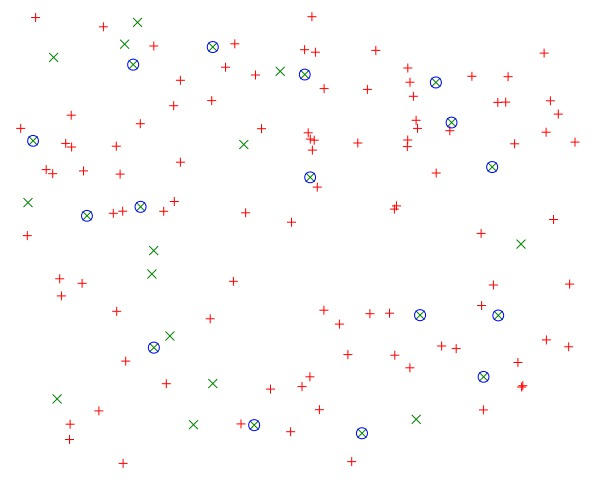
\includegraphics[scale=0.35]{Test_100_30_16_16}\caption{n = 100, m = 30, p = 16, l = 16}}\end{figure}}
